\documentclass[../Cours.tex]{subfiles}

\usepackage{xstring}
\usepackage{xfp}

\begin{document}
\clearpage
\thispagestyle{empty}

\color{black}
\nomPrenom
\titreDScorrection

\begin{questions}
    \EXERCICETITRE{3}{Nombres relatifs}
    \question Classer ces évènements \textit{du plus ancien au plus récent}.\vspace{-1em}
        \begin{multicols}{2}
        \subquestion Fondation de Rome : -753
        \subquestion Fin de la guerre d'Algérie : 1962
        \subquestion Mort d'Aristote : -322
        \subquestion Sacre de Louis XIV : 1654
        \subquestion Coup d'état du 18 brumaire : 1799
        \subquestion Mort de Jules César : -44
        \end{multicols} 

    {\color{rouge}
    Fondation de Rome < Mort d'Aristote < Mort de Jules César < Sacre de Louis XIV < Coup d'état du 18 brumaire < Fin de la guerre d'Algérie\\ 
    \[ -753 < -322 < -44 < 1654 < 1799 < 1962 \]
    }
    
    \question La magnitude d'un objet représente sa brillance. Plus la magnitude est grande, moins l'objet est brillant. Classer ces objets célestes \textit{dans l'ordre croissant} de leur magnitude.\vspace{-1em}
        \begin{multicols}{3}
        \subquestion ISS : \num{-4.5}
        \subquestion Soleil : \num{-26.7}
        \subquestion Vénus : -4
        \subquestion Saturne : \num{-0.4}
        \subquestion Véga : 0
        \subquestion Sirius : \num{-1.4}
        \end{multicols}
    
    {\color{rouge}
    Soleil < ISS (\textit{International Space Station}) < Vénus < Sirius < Saturne < Véga \\ 
    \[ -26{,}7 < -4{,}5 < -4 < -1{,}4 < -0{,}4 < 0 \]
    }

    \EXERCICETITRE{4}{Parallélogrammes}
    \question Donner et justifier la nature de ce quadrilatère.

    \begin{centre}
        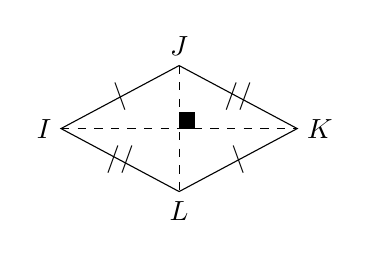
\begin{tikzpicture}
            %\draw (0,0) node[below]{$A$} -- +(1,2) node[left]{$B$}  node[midway]{\_}-- +(4,2) node[right]{$C$}  node[midway]{//}-- +(3,0) node[below]{$D$}  node[midway]{\_}-- cycle node[midway]{//};
            %\draw (6,0) node[below]{$E$} -- +(0,2.5) node[above]{$F$} node[midway]{\_} -- +(1.5,2.5) node[above]{$G$} node[midway]{//} -- +(1.5,0) node[below]{$H$} node[midway]{\_} -- cycle node[midway]{//};
            %\filldraw (6,2.5) rectangle +(0.2,-0.2);
            \draw (-1.5,1) node[left]{$I$} -- +(1.5,0.8) node[above]{$J$} node[midway]{\textbackslash} -- +(3,0) node[right]{$K$} node[midway]{//} -- +(1.5,-0.8) node[below]{$L$} node[midway]{\textbackslash} -- cycle node[midway]{//};
            \draw[dashed] (-1.5,1) -- +(3,0);
            \draw[dashed] (0,1.8) -- +(0,-1.6);
            \filldraw (0,1) rectangle +(0.2,0.2);
        \end{tikzpicture}
    \end{centre}

    {\color{rouge}
        \underline{On sait que :} $IJKL$ est un quadrilatère, $IJ=KL$ et $JK=IL$\\
        \underline{Or : } Si un quadrilatère a ses côtés opposés de même longueur, alors c'est un parallélogramme.\\
        \underline{Donc :} $IJKL$ est un parallélogramme.\\

        \underline{On sait que :} $IJKL$ est un parallélogramme et $(IK)\perp(JL)$\\
        \underline{Or : } Si les diagonales d'un parallélogramme sont perpendiculaires, alors c'est un losange.\\
        \underline{Donc :} $IJKL$ est un losange.
    }

    \clearpage
    \EXERCICETITRE{4}{Cuire des pâtes}
    Pour saler l'eau des pâtes, il est recommandé d'utiliser \textbf{\qty{10}{\gram} de sel pour \qty{1}{\litre} d'eau.}
    \question En tant que chef cuisinier, vous prélevez de l'eau de cuisson de votre apprenti pour vérifier qu'il a bien respecter la règle. Dans \qty{20}{\ml} d'eau, il y a \qty{150}{\milli\gram} de sel, est-ce suffisant ?

    {\color{rouge}
    \begin{center}
        La valeur de référence est de \qty{10}{\gram\per\litre}.\\
        On a \qty{150}{\milli\gram} de sel pour \qty{20}{\milli\litre} d'eau.\\
        $\dfrac{\qty{150}{\milli\gram}}{\qty{20}{\milli\litre}} = \qty{7.5}{\gram\per\litre}$\\
        Il s'agit donc d'une concentration inférieure aux \qty{10}{\gram\per\litre} : c'est insuffisant.
    \end{center}        
    }
    
    \question En respectant la règle de \qty{10}{\gram\per\litre}, quelle quantité de sel faut-il pour \qty{4}{\litre} d'eau de cuisson ?

    {\color{rouge}
    \begin{center}
        \begin{tabularx}{0.5\linewidth}{|l|X|X|}\hline
            Masse de sel (\unit{\gram}) & 10 & ? \\\hline
            Quantité d'eau (\unit{\litre}) & 1 & 4 \\\hline
        \end{tabularx}\\
        
        Par un produit en croix, on trouve $\dfrac{10 \times 4}{1} = \qty{40}{\gram}$.
    \end{center}
    }
    
    \question Pour faire cuire l'eau des pâtes, on a besoin d'une casserole. Ici, on suppose qu'elle a la forme d'un cylindre de \qty{12}{\centi\metre} de rayon, et de \qty{10}{\centi\metre} de hauteur.
        \subquestion Quel est le volume de ce cylindre ? (rappel : $V_{\mbox{cylindre}} = \pi r^2 h$)

        {\color{rouge}
            On calcule le volume du cylindre en utilisant la formule :
            \begin{align*}
                V_{\mbox{cylindre}} &= \pi r^2 h \\
                &= \pi \times (\qty{12}{\centi\metre})^2 \times \qty{10}{\centi\metre} \\
                &\approx \boxed{\qty{4523.89}{\centi\metre\cubed}}
            \end{align*}
        }
        
        \subquestion Cette casserole est-elle assez grande pour cuire \qty{3}{\litre} d'eau ?

        {\color{rouge}
            Ici, on a besoin de savoir si les \qty{3}{\litre} d'eau rentre dans la casserole de volume \qty{4523.89}{\centi\metre\cubed}. Mais ces deux valeurs n'ont pas les mêmes unités, il faut donc convertir.\\
            On sait que $\qty{1}{\litre} = \qty{1}{\deci\metre\cubed}$ et $\qty{1}{\deci\metre\cubed} = \qty{1000}{\centi\metre\cubed}$.\\
            \begin{align*}
                \qty{4523.89}{\centi\metre\cubed} &= \qty{4.52389}{\deci\metre\cubed} \\
                &= \qty{4.52389}{\litre}\\
                &\approx \qty{4.5}{\litre}
            \end{align*}
            La casserole est donc suffisamment grande pour faire cuire \qty{3}{\litre} d'eau.
        }
    \clearpage
    \EXERCICETITRE{7}{Diagrammes}
    On s'intéresse à l'évolution de la population de la ville de Paris du Moyen-Âge à nos jours. Le tableau ci-dessous donne le nombre d'habitants à Paris entre l'année 1220 et 2020 :
    \begin{center}
        \begin{flushright}
            \textit{En millions d'habitants}
        \end{flushright}
        \begin{tabularx}{0.9\linewidth}{|l|X|X|X|X|X|X|X|}\hline
            Année & 1220 & 1680 & 1811 & 1901 & 1962 & 2020  \\\hline
            Nombre d'habitants & \num{50000} & \num{500000} & \num{622636} & \num{2714068} & \num{2790091} & \num{2145906} \\\hline
        \end{tabularx}
        \begin{flushright}\vspace{-0.8em}
            \textit{(source INSEE)}
        \end{flushright}
    \end{center}

    \question Compléter le diagramme en barres ci-dessous : 
    \begin{center}
        \begin{tikzpicture}[xscale=1.6,yscale=0.8]
            \draw[-Latex] (0,0) -- (10.5,0);
            \draw[-Latex] (0,0) -- (0,7);
            \foreach \x in {1.5,3,...,9} {
                \draw (\x,-0.2) -- (\x,0.2);
            }
            \node[below] at (1.5,-0.2) {1220};
            \node[below] at (3,-0.2) {1680};
            \node[below] at (4.5,-0.2) {1811};
            \node[below] at (6,-0.2) {1901};
            \node[below] at (7.5,-0.2) {1962};
            \node[below] at (9,-0.2) {2020};
            \foreach \y in {0,1,...,3} {
                \draw[gray] (0,{2*\y}) -- +(10.5,0);
                \node[left] at (0,{2*\y}) {\small{\y}};
            }
            \foreach \i in {0,1,2} {
                \foreach \y in {0.1,0.2,...,0.9} {
                    \draw[gray!40!white] (0,{2*(\i+\y)}) -- +(10.5,0);
                }
            }
            \filldraw (1.2,0) rectangle (1.8,{2*0.05});
            \filldraw (2.7,0) rectangle (3.3,{2*0.5});
            \filldraw (8.7,0) rectangle (9.3,{2*2.145906});
            \filldraw[rouge] (4.2,0) rectangle (4.8,{2*0.622636});
            \filldraw[rouge] (5.7,0) rectangle (6.3,{2*2.714068});
            \filldraw[rouge] (7.2,0) rectangle (7.7,{2*2.790091});
        \end{tikzpicture}
    \end{center}

    On s'intéresse maintenant à la répartition des habitant de Paris en 2019 selon leur tranche d'âge :  
    \begin{center}
        \begin{tabularx}{0.8\linewidth}{|l|X|X|}\hline
        Tranche d'âge & Nombre d'habitants & Degrés (arrondi à l'unité) \\\hline\hline
        0-14 ans & \num{317777} & \textcolor{rouge}{\ang{52}} \\\hline
        15-29 ans & \num{520988} & \textcolor{rouge}{\ang{85}} \\\hline
        30-44 ans & \num{530442} & \textcolor{rouge}{\ang{86}} \\\hline
        45-59 ans & \num{414786} & \textcolor{rouge}{\ang{68}} \\\hline
        60-74 ans & \num{263008} & \textcolor{rouge}{\ang{43}} \\\hline
        75 ans et + & \num{164296} & \textcolor{rouge}{\ang{27}} \\\hline
        Total & \num{2211297} & \textbf{\ang{360}} \\\hline
        \end{tabularx}
        \begin{flushright}\vspace{-0.8em}
            \textit{(source INSEE : \tiny{https://www.insee.fr/fr/statistiques/6455183?sommaire=6455209\&geo=DEP-75})}
        \end{flushright}
    \end{center}

    \question Compléter le tableau pour calculer les angles nécessaires au diagramme circulaire.
    \question Compléter le diagramme circulaire ci-dessous : 
    \begin{center}
        \begin{tikzpicture}[scale=0.9]
            \draw (0,0) circle (2.7);
            \draw (0,0) -- (2.7,0);
            \foreach \i/\c in {1/rouge,2/vert,3/bleu,4/jaune,5/orange,6/noir} {
                \draw[fill=\c] (4,{2.5 - \i*0.7}) rectangle +(0.3,0.3);
                \draw (4.4,{2.5 - \i*0.7}) -- +(6,0);
            }
            \node[anchor=west,rouge] at (4.6,{2.75 - 1*0.7}) {0-14 ans};
            \node[anchor=west,rouge] at (4.6,{2.75 - 2*0.7}) {15-29 ans};
            \node[anchor=west,rouge] at (4.6,{2.75 - 3*0.7}) {30-44 ans};
            \node[anchor=west,rouge] at (4.6,{2.75 - 4*0.7}) {45-59 ans};
            \node[anchor=west,rouge] at (4.6,{2.75 - 5*0.7}) {60-74 ans};
            \node[anchor=west,rouge] at (4.6,{2.75 - 6*0.7}) {75 ans et +};
            \filldraw[rouge] (0,0) -- ({2.7*cos(0)},{2.7*sin(0)}) arc(0:52:2.7) -- cycle;
            \filldraw[vert] (0,0) -- ({2.7*cos(52)},{2.7*sin(52)}) arc(52:52+85:2.7) -- cycle;
            \filldraw[bleu] (0,0) -- ({2.7*cos(52+85)},{2.7*sin(52+85)}) arc(52+85:52+85+86:2.7) -- cycle;
            \filldraw[jaune] (0,0) -- ({2.7*cos(52+85+86)},{2.7*sin(52+85+86)}) arc(52+85+86:52+85+86+68:2.7) -- cycle;
            \filldraw[orange] (0,0) -- ({2.7*cos(52+85+86+68)},{2.7*sin(52+85+86+68)}) arc(52+85+86+68:52+85+86+68+43:2.7) -- cycle;
            \filldraw[noir] (0,0) -- ({2.7*cos(52+85+86+68+43)},{2.7*sin(52+85+86+68+43)}) arc(52+85+86+68+43:52+85+86+68+43+27:2.7) -- cycle;
        \end{tikzpicture}
    \end{center}
\end{questions}
\end{document}